\chapter{Photographs of the First Road Session}
\label{app:road1}

These photographs and video stills were taken by the team around the first road session of 19 October 2026 (Section~\ref{sec:field-test-design}) and shared on 21 October. The originals, twelve photographs and five short videos, are kept in the project's \texttt{Roadtest1} folder and not in the repository. In line with Section~\ref{sec:ethics}, the faces of other people have been cropped away or blurred and the vehicle's number plate blurred; the videos show people, so they are listed in Table~\ref{tab:road1-videos} rather than reproduced.

\section{Rear sensor pod}

Figure~\ref{fig:road1-pod} shows the rear sensor pod of Appendix~\ref{app:mechanical} as built: the camera head with the time-of-flight board, the Raspberry Pi~4 with its fan and the ESP32 telemetry unit in their bays, and the vented lid with its push-on hood.

\begin{figure}[H]
\centering
\subfigure[Open, from above: the bays with the Raspberry Pi~4 and the ESP32, a battery pack held in the lid, and the head tray with the time-of-flight board below.]{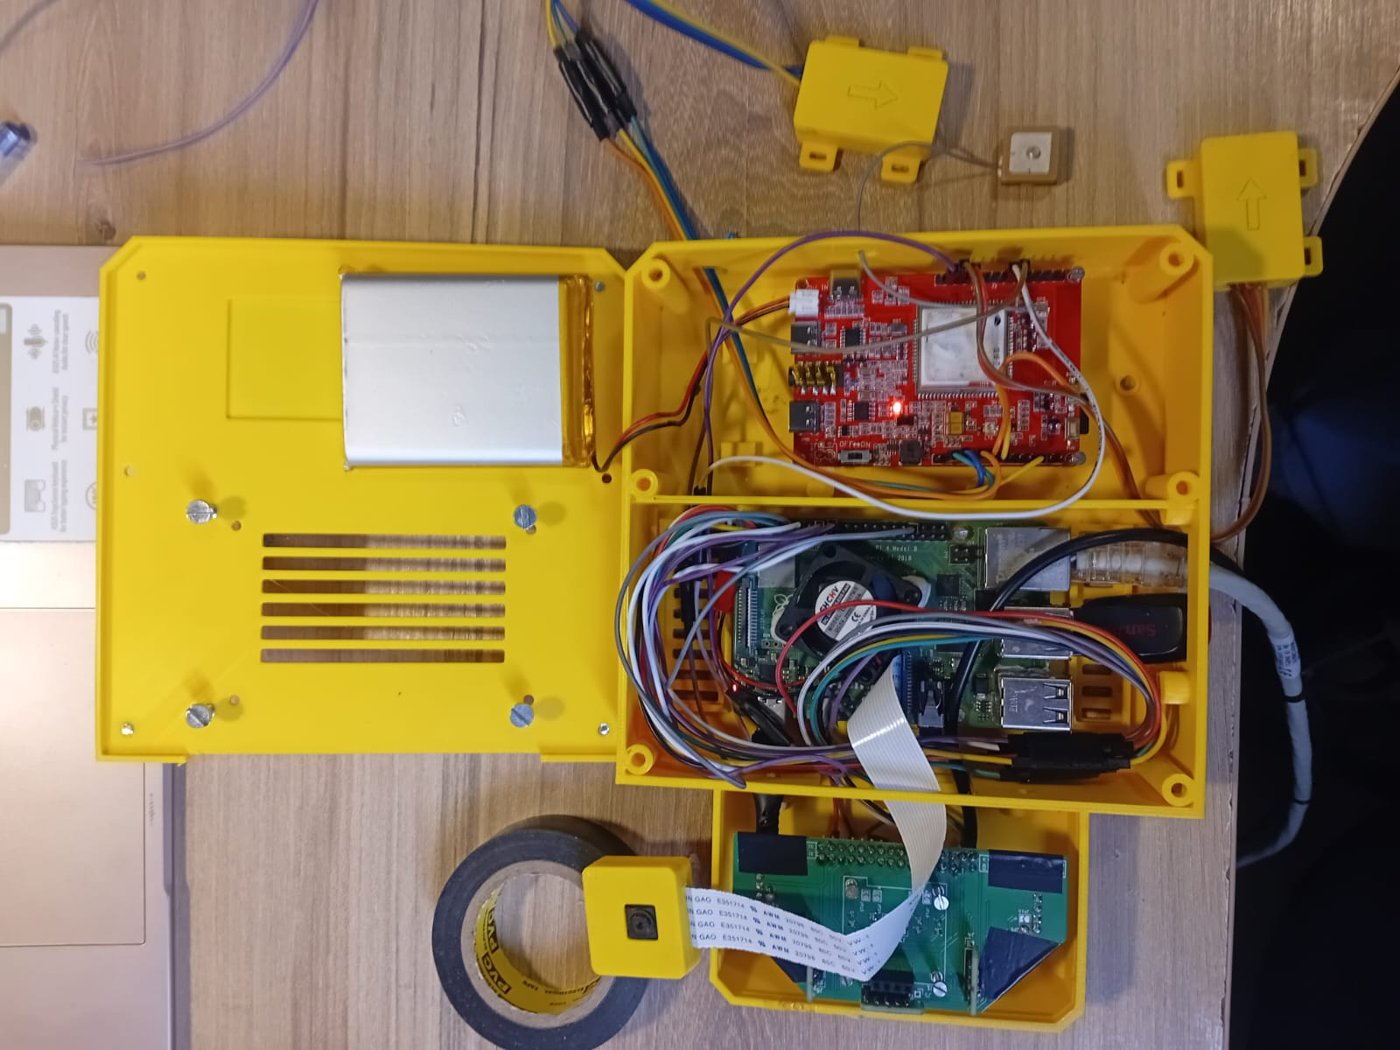
\includegraphics[width=0.42\textwidth]{figures/road1/pod_open_top.jpg}}
\hfill
\subfigure[Open, with the camera head lifted on its ribbon cable beside the time-of-flight board.]{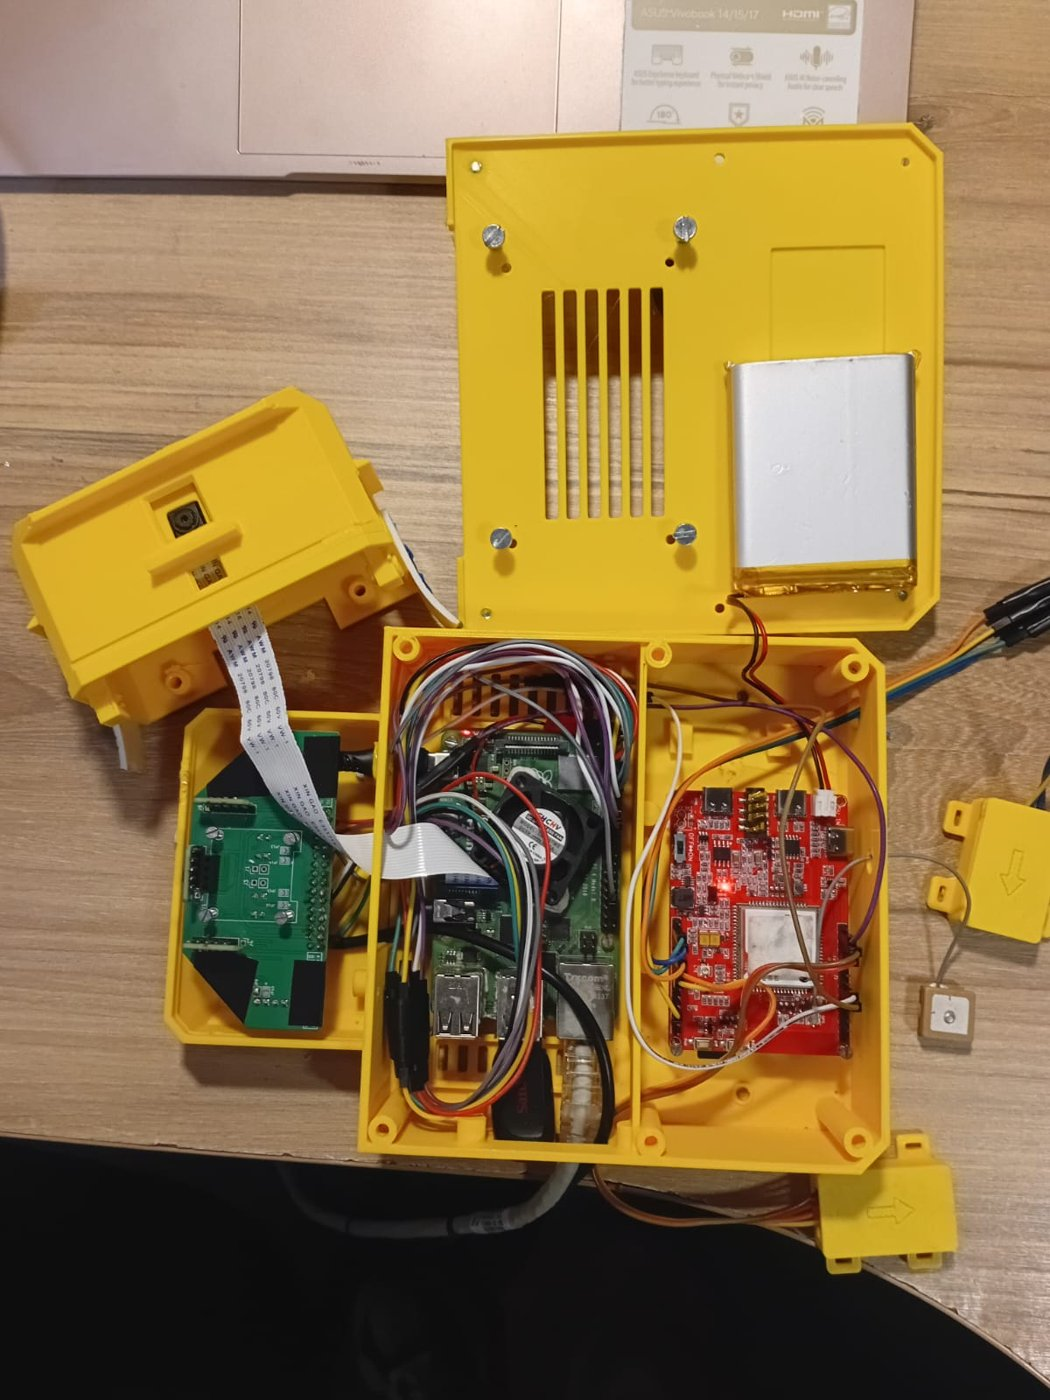
\includegraphics[width=0.31\textwidth]{figures/road1/pod_open_bays.jpg}}
\\[4pt]
\subfigure[Closed, with the hood over the lid's exhaust grille and the head tray open at the front.]{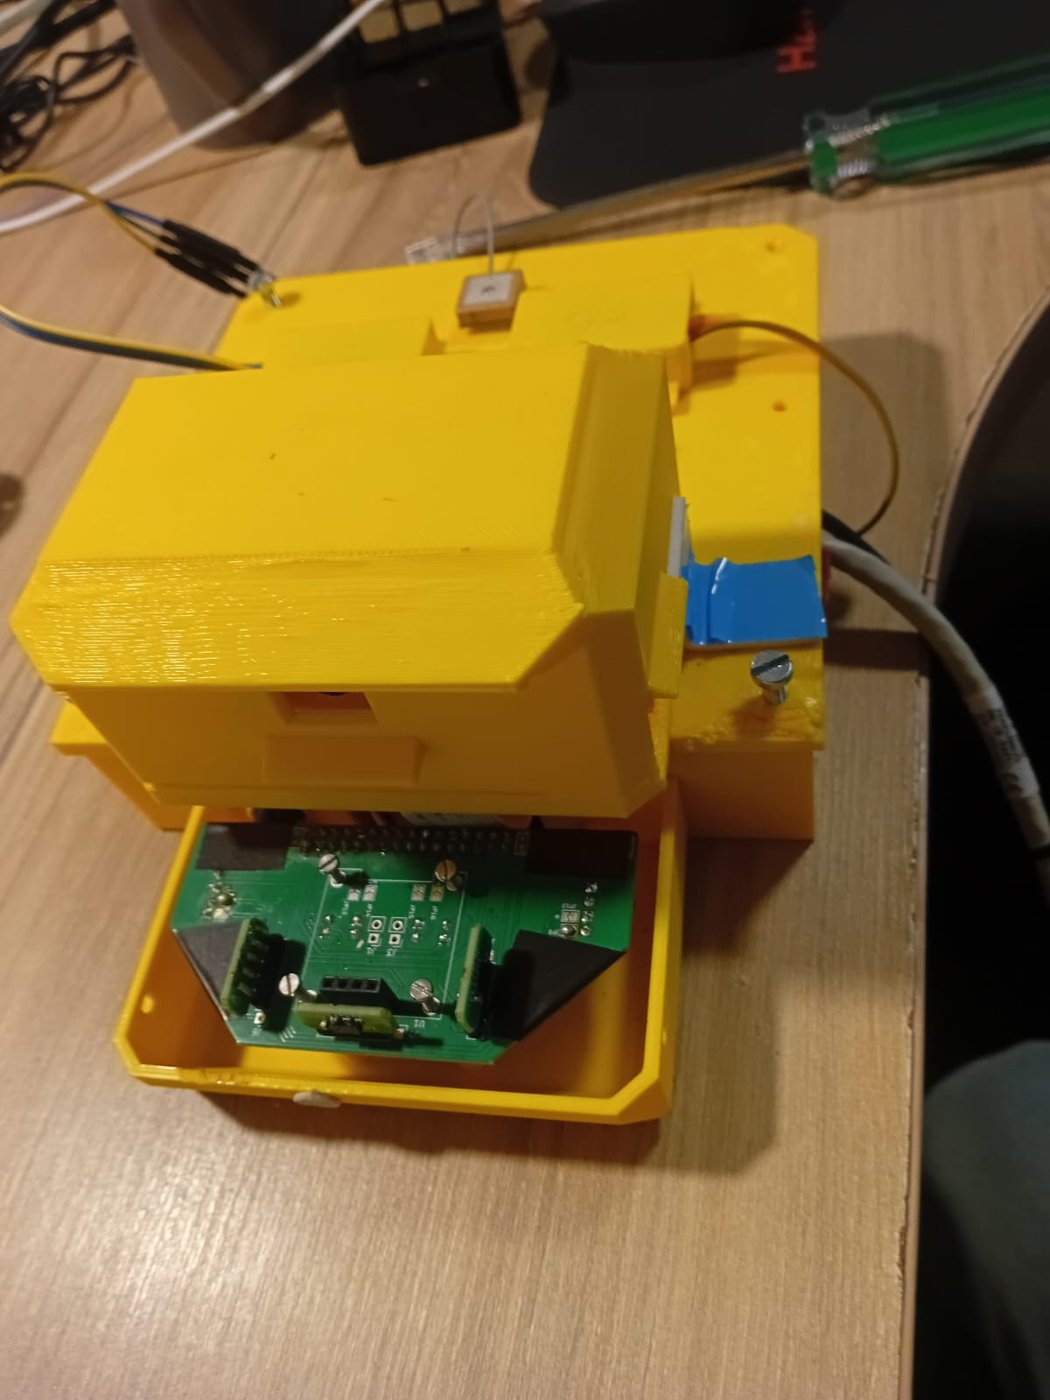
\includegraphics[width=0.31\textwidth]{figures/road1/pod_closed_hood.jpg}}
\hfill
\subfigure[The lid from above, with the GNSS antenna on top and the grille under the hood.]{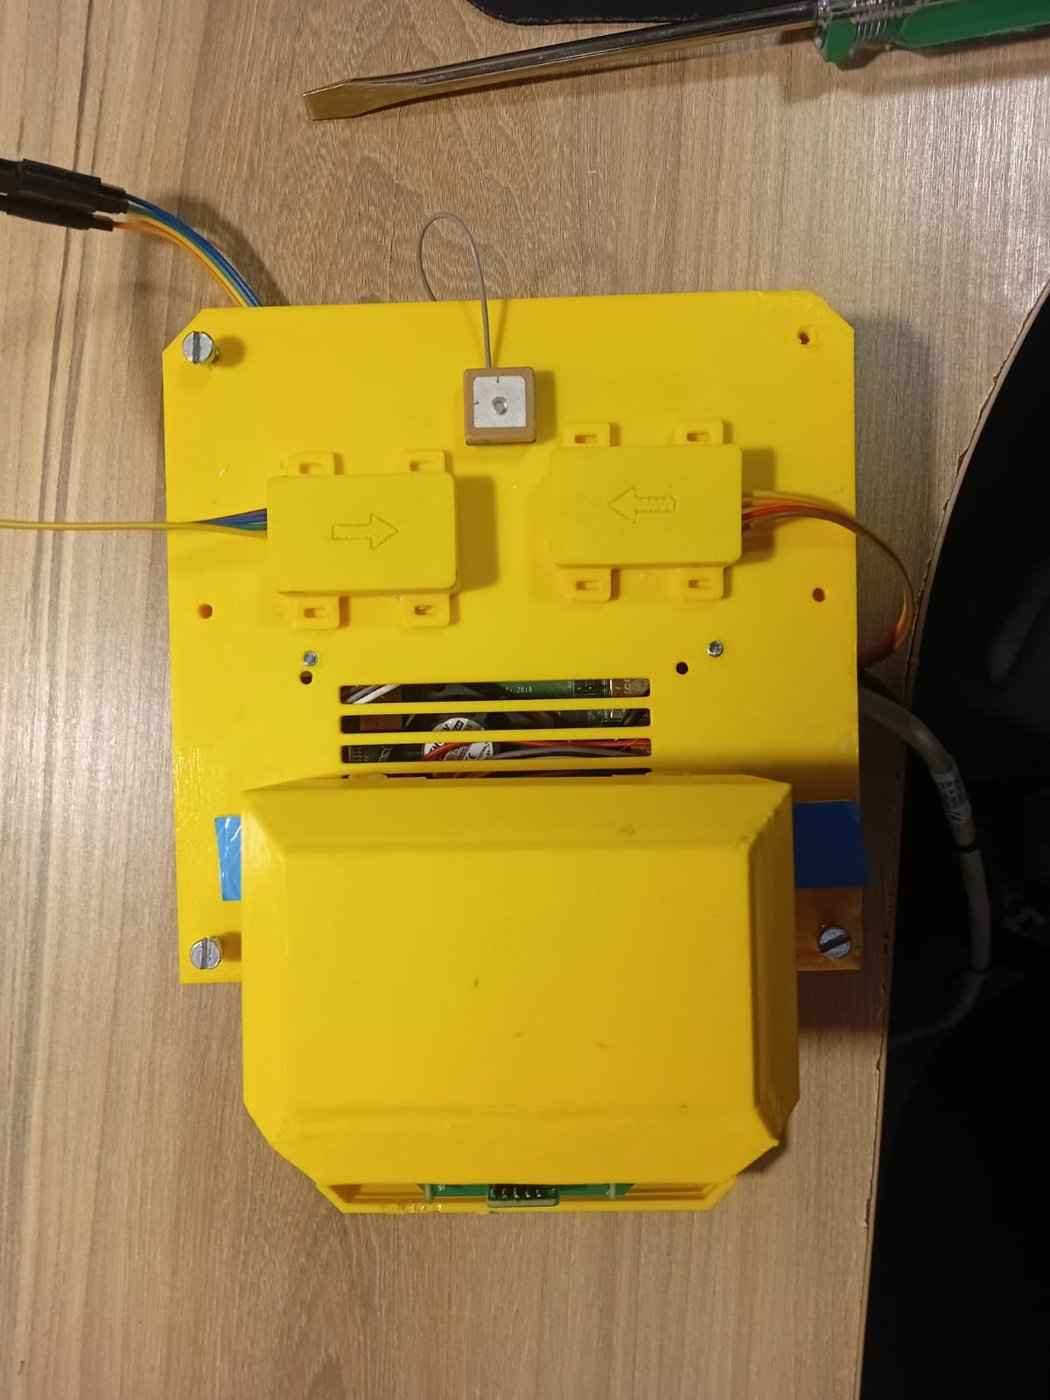
\includegraphics[width=0.31\textwidth]{figures/road1/pod_lid_antenna.jpg}}
\caption{The rear sensor pod, printed and assembled.}
\label{fig:road1-pod}
\end{figure}

\clearpage
\section{The system on the vehicle}

Figure~\ref{fig:road1-vehicle} shows the units mounted over the rear frame of the TUKZIE Rev 0, outdoors and in the laboratory, with the removable mounting of R13: a board laid over the frame and the units on it, with no drilling.

\begin{figure}[H]
\centering
\subfigure[From behind: the rear sensor pod (yellow) at the back edge of the board, the small IMU pods, and the power strip at the front of the bed.]{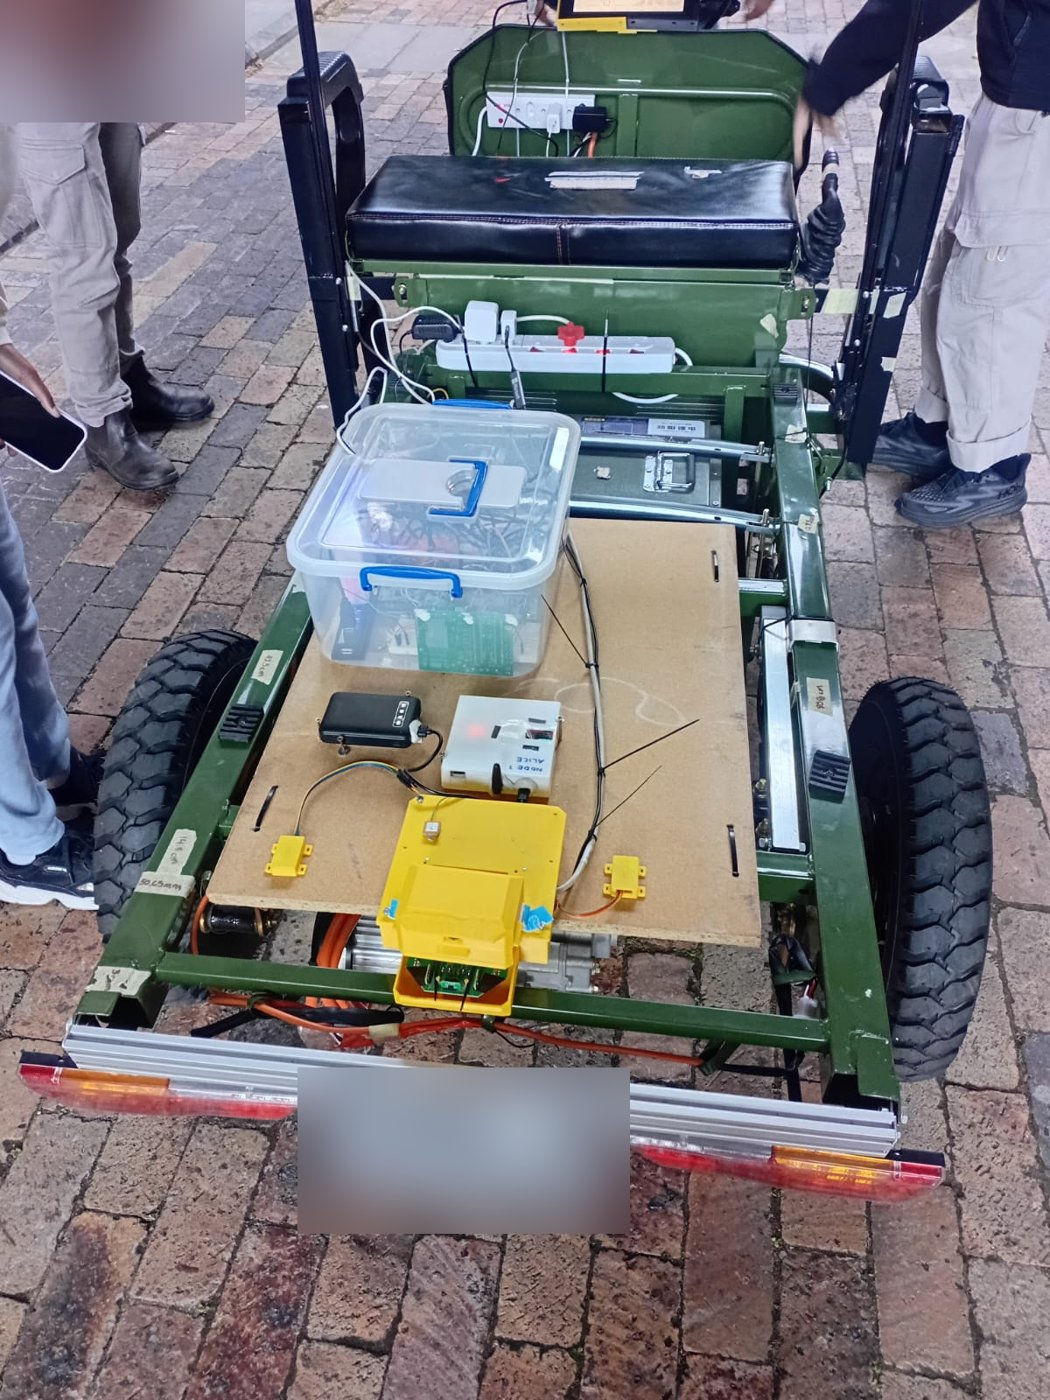
\includegraphics[width=0.31\textwidth]{figures/road1/chassis_rear.jpg}}
\hfill
\subfigure[Closer, with a clear box holding further electronics and the units on the board.]{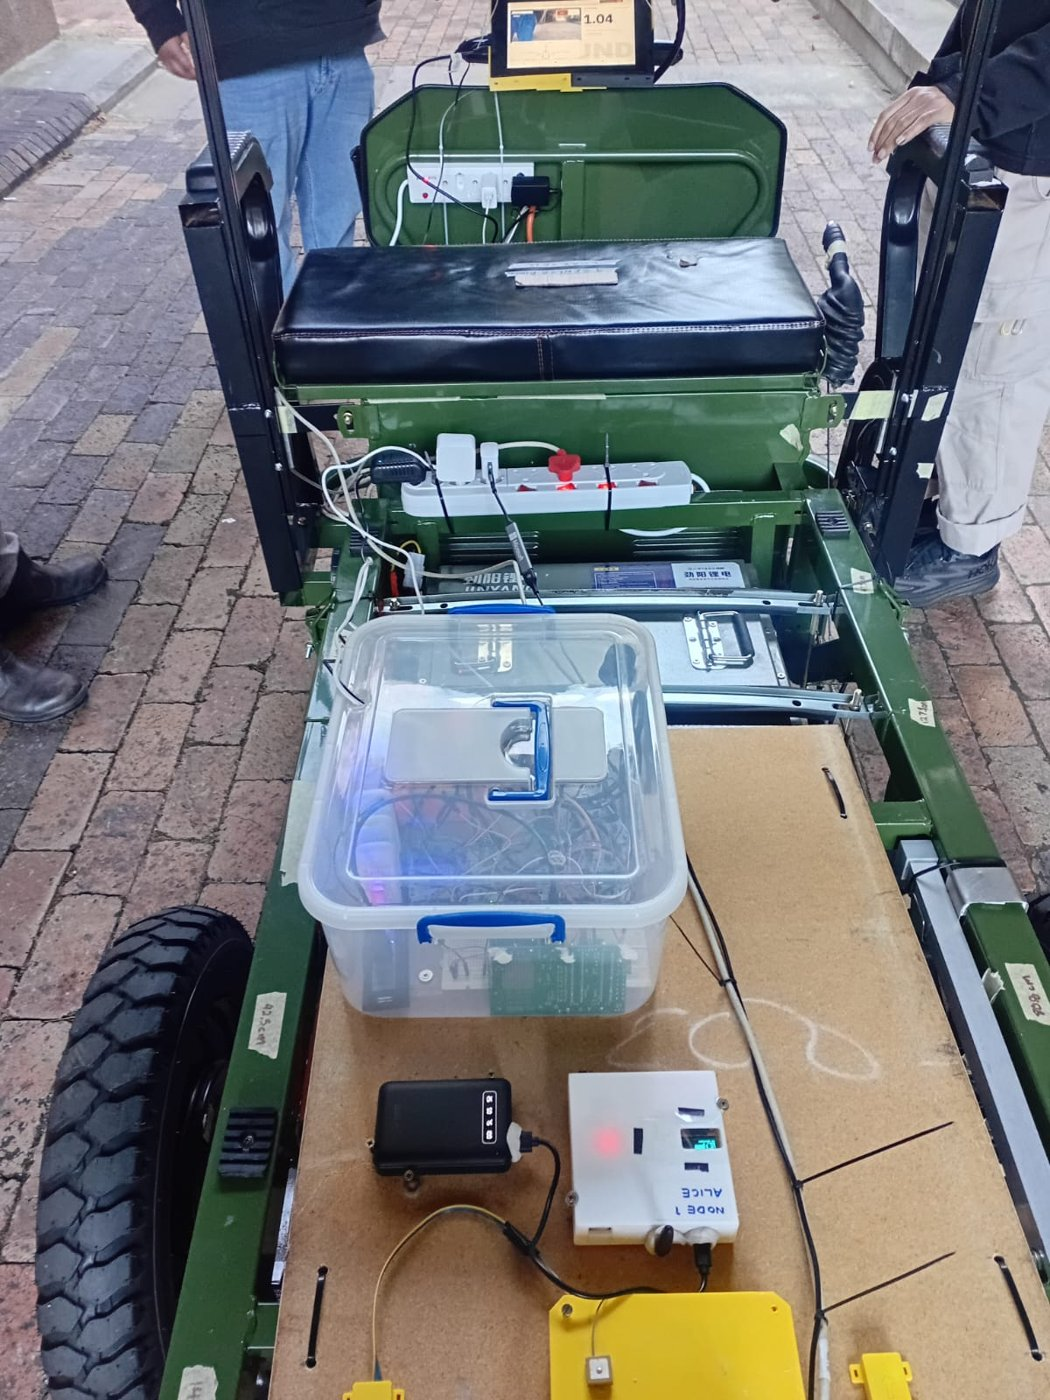
\includegraphics[width=0.31\textwidth]{figures/road1/chassis_rear_close.jpg}}
\\[4pt]
\subfigure[The whole vehicle from behind, outdoors.]{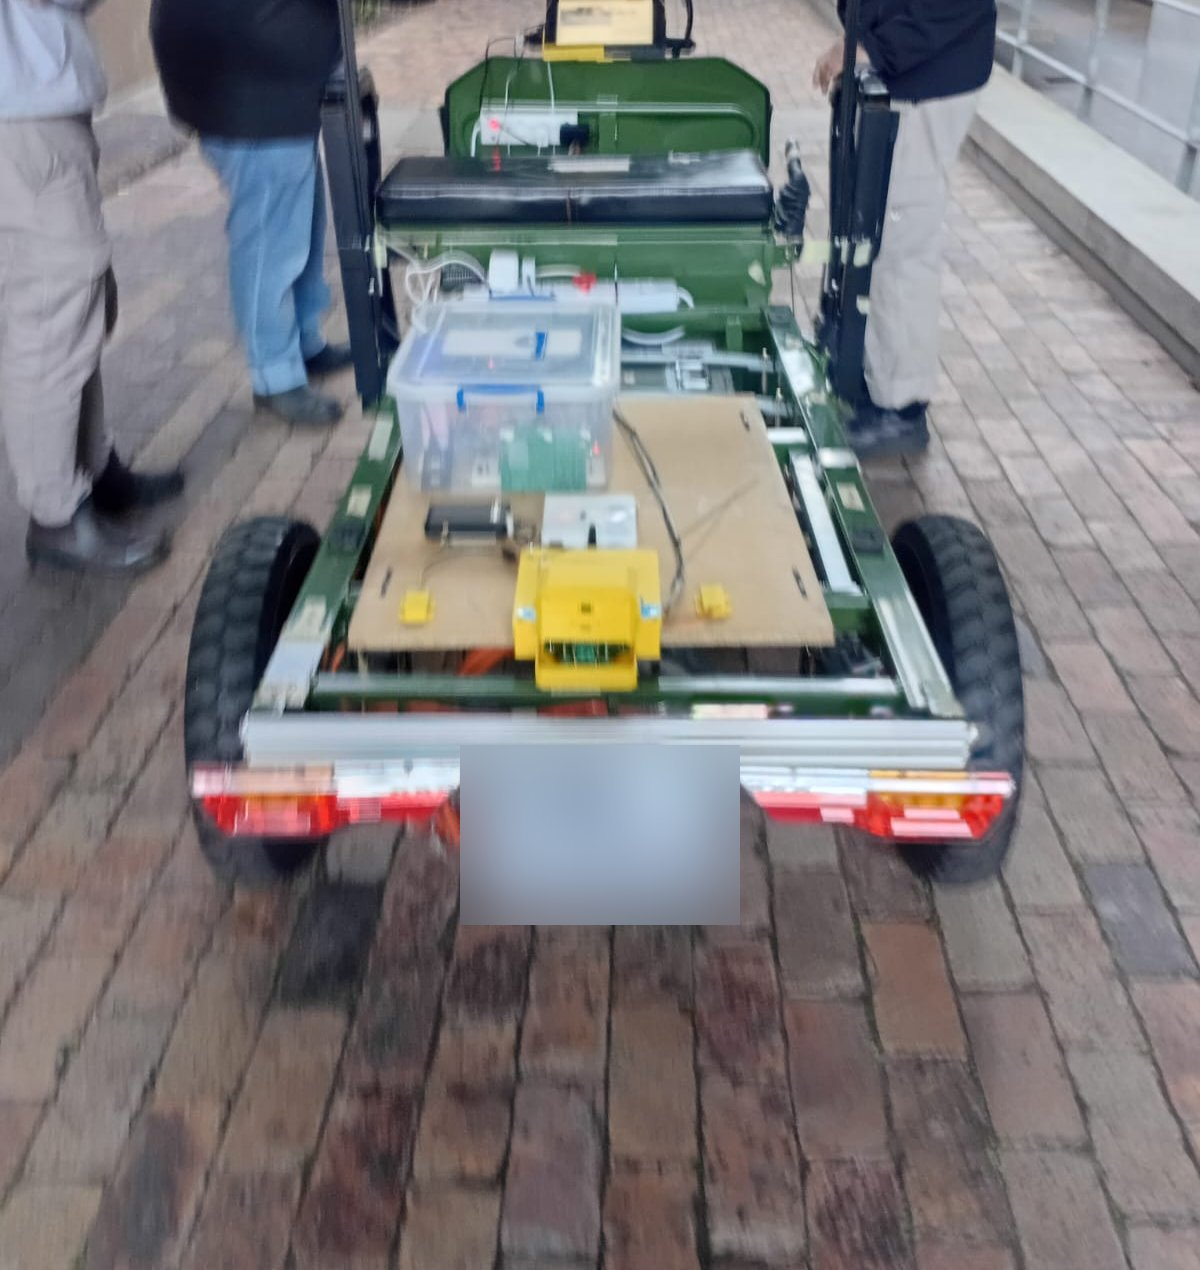
\includegraphics[width=0.31\textwidth]{figures/road1/chassis_rear_wide.jpg}}
\hfill
\subfigure[From the side in the laboratory (video still).]{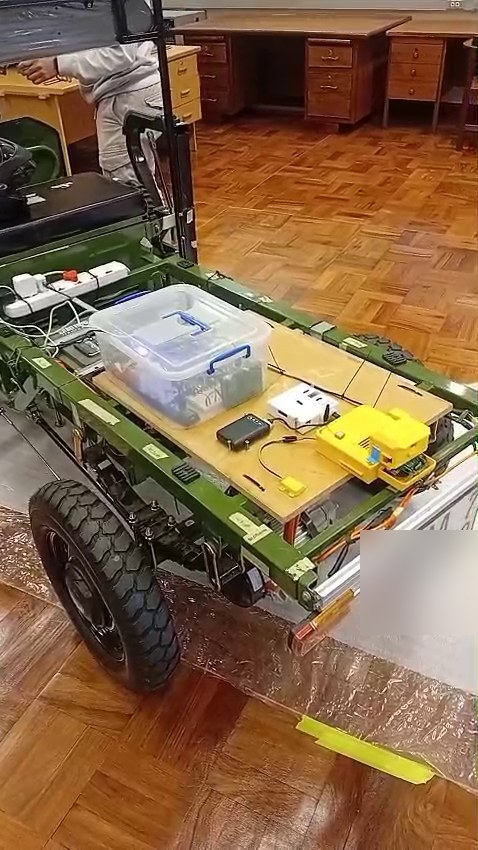
\includegraphics[width=0.30\textwidth]{figures/road1/vid_chassis_side.jpg}}
\caption{The system mounted on the vehicle. Faces and the number plate are blurred or cropped.}
\label{fig:road1-vehicle}
\end{figure}

\clearpage
\section{The dashboard on the handlebar}

Figure~\ref{fig:road1-dash} shows the display in its printed holder on the handlebar, with the dashboard running.

\begin{figure}[H]
\centering
\subfigure[The display on the handlebar, outdoors.]{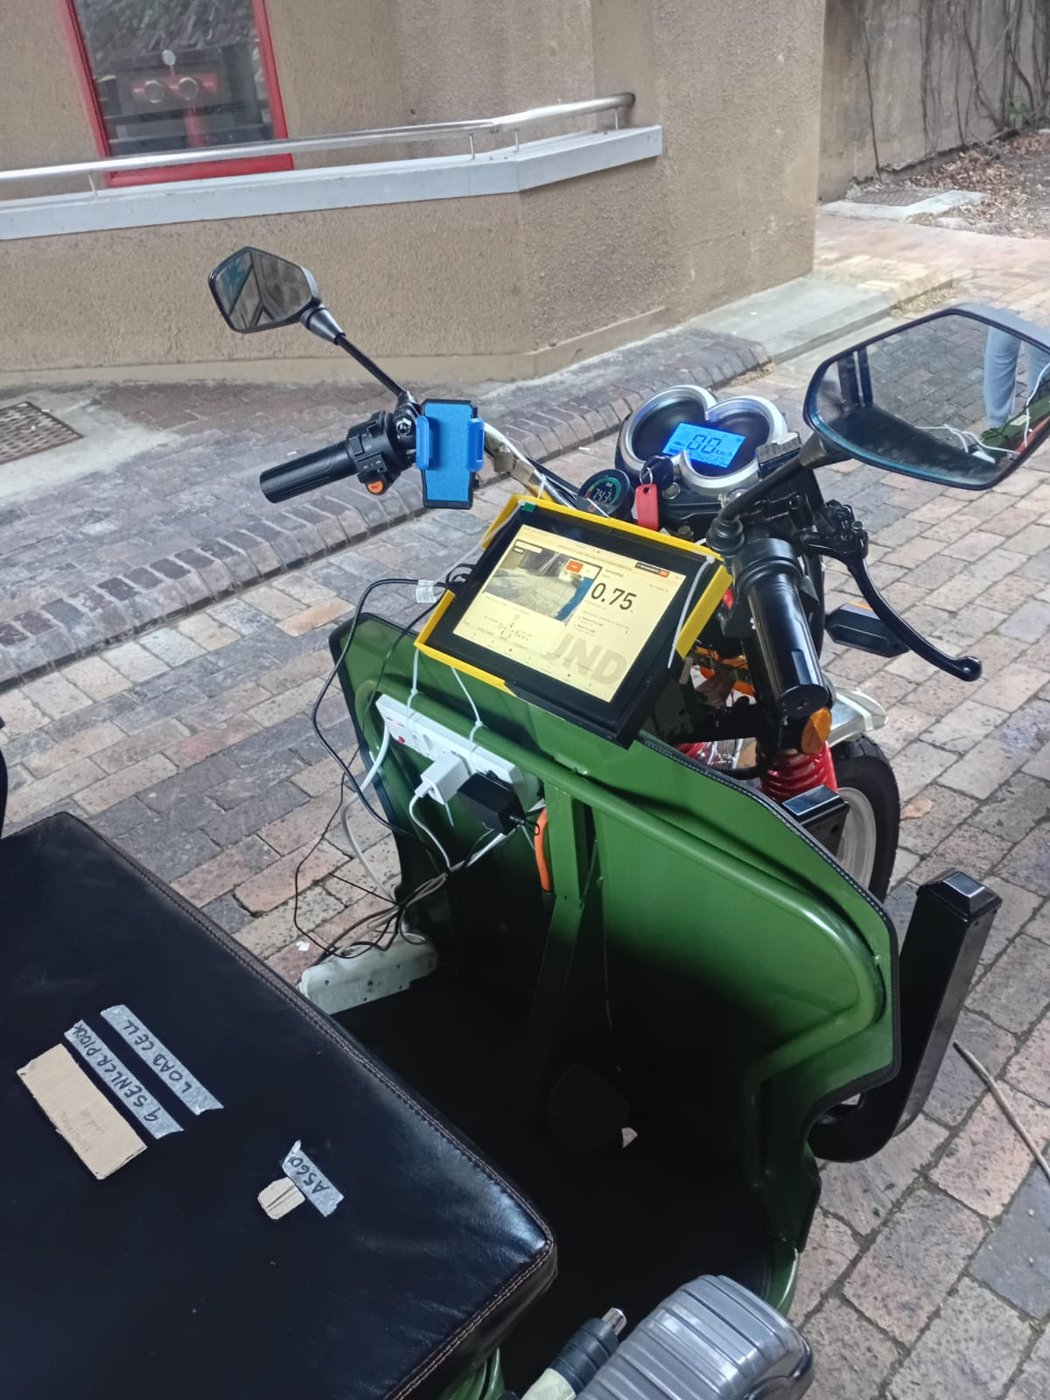
\includegraphics[width=0.30\textwidth]{figures/road1/dash_on_bar.jpg}}
\hfill
\subfigure[From the seat.]{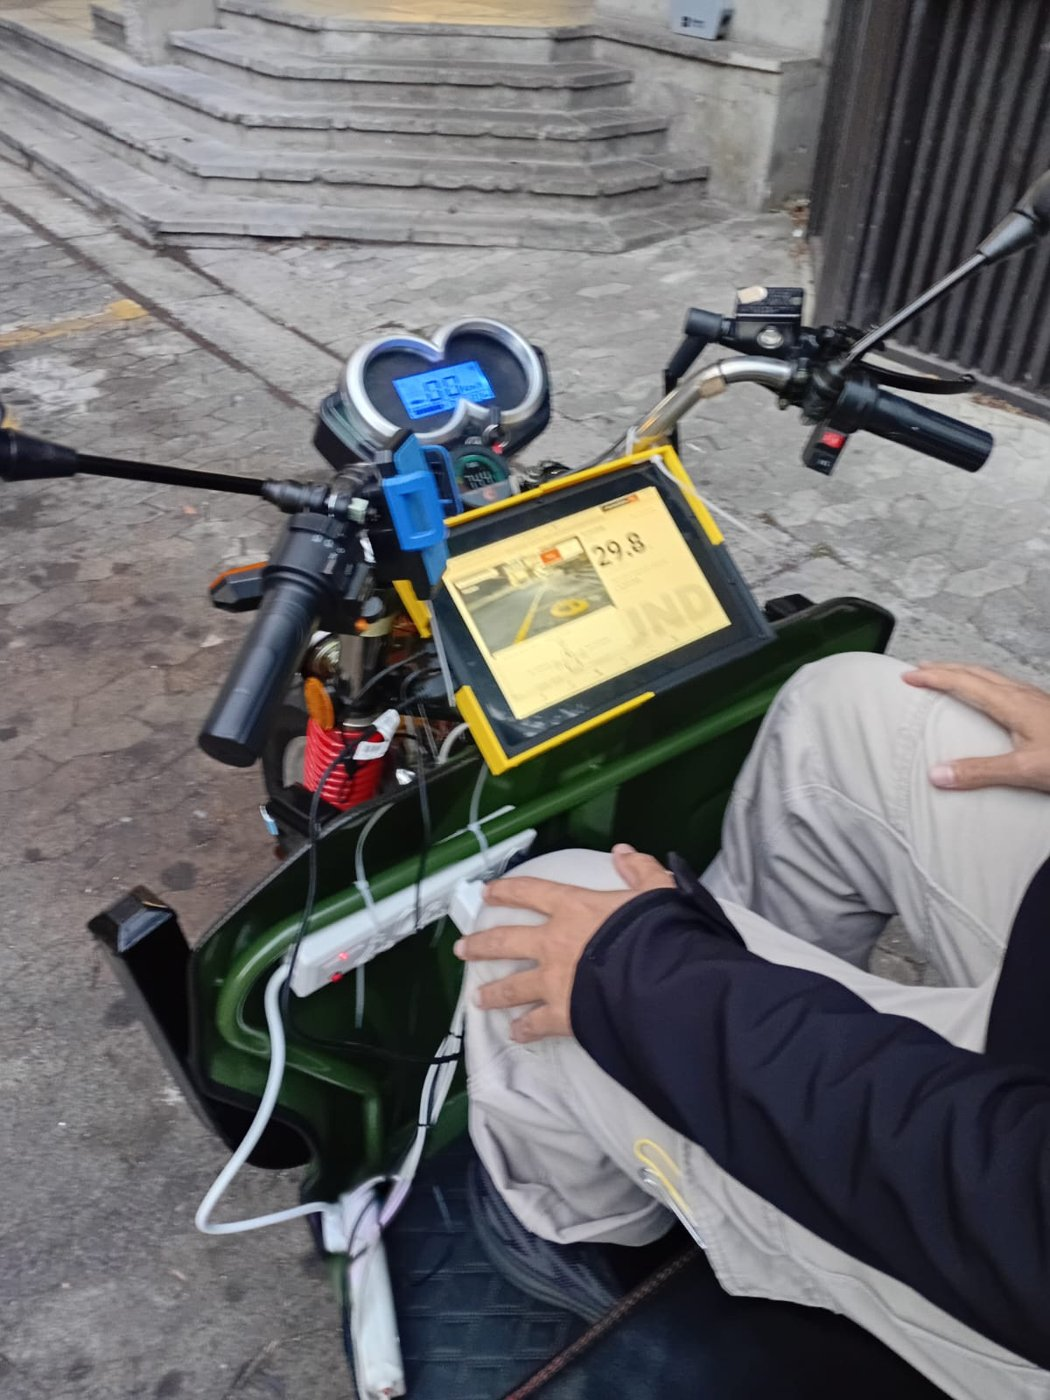
\includegraphics[width=0.30\textwidth]{figures/road1/dash_on_bar_seated.jpg}}
\hfill
\subfigure[The DRIVE page (video still).]{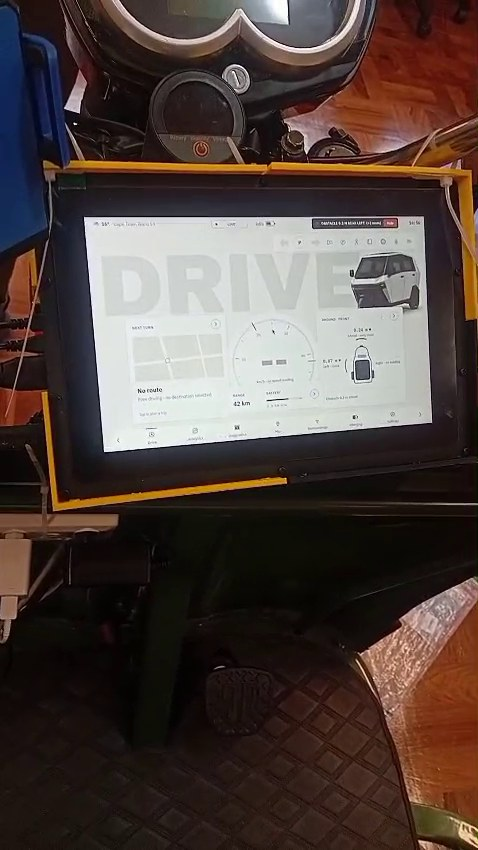
\includegraphics[width=0.30\textwidth]{figures/road1/vid_dash_drive.jpg}}
\caption{The dashboard display mounted on the vehicle.}
\label{fig:road1-dash}
\end{figure}

\begin{table}[htbp]
\centering
\small
\caption{Videos from the first road session, kept with the originals (file names as shared on 21 October 2026).}
\label{tab:road1-videos}
\begin{tabular}{|p{4.6cm}|p{1.2cm}|p{8.0cm}|}
\hline
\textbf{File} & \textbf{Length} & \textbf{What it shows} \\ \hline
WhatsApp Video 2026-10-21 at 21.07.44 & 45\,s & From a corridor to a doorway as the vehicle is ridden out of the building \\ \hline
WhatsApp Video 2026-10-21 at 21.07.53 & 19\,s & A toy RC car and its remote shown to the camera, then the vehicle pushed through a doorway into a lecture venue \\ \hline
WhatsApp Video 2026-10-21 at 21.08.18 & 8\,s & A walk round the rear frame with the units mounted, indoors \\ \hline
WhatsApp Video 2026-10-21 at 21.08.19 & 16\,s & The vehicle ridden slowly inside the lecture venue \\ \hline
WhatsApp Video 2026-10-21 at 21.08.20 & 43\,s & The wiring at the bed, then the display on the handlebar showing the DRIVE page \\ \hline
\end{tabular}
\end{table}
